\documentclass[]{article}
\usepackage{lmodern}
\usepackage{amssymb,amsmath}
\usepackage{ifxetex,ifluatex}
\usepackage{fixltx2e} % provides \textsubscript
\ifnum 0\ifxetex 1\fi\ifluatex 1\fi=0 % if pdftex
  \usepackage[T1]{fontenc}
  \usepackage[utf8]{inputenc}
\else % if luatex or xelatex
  \ifxetex
    \usepackage{mathspec}
    \usepackage{xltxtra,xunicode}
  \else
    \usepackage{fontspec}
  \fi
  \defaultfontfeatures{Mapping=tex-text,Scale=MatchLowercase}
  \newcommand{\euro}{€}
\fi
% use upquote if available, for straight quotes in verbatim environments
\IfFileExists{upquote.sty}{\usepackage{upquote}}{}
% use microtype if available
\IfFileExists{microtype.sty}{\usepackage{microtype}}{}
\usepackage[margin=1in]{geometry}
\usepackage{color}
\usepackage{fancyvrb}
\newcommand{\VerbBar}{|}
\newcommand{\VERB}{\Verb[commandchars=\\\{\}]}
\DefineVerbatimEnvironment{Highlighting}{Verbatim}{commandchars=\\\{\}}
% Add ',fontsize=\small' for more characters per line
\newenvironment{Shaded}{}{}
\newcommand{\AlertTok}[1]{\textcolor[rgb]{1.00,0.00,0.00}{\textbf{#1}}}
\newcommand{\AnnotationTok}[1]{\textcolor[rgb]{0.38,0.63,0.69}{\textbf{\textit{#1}}}}
\newcommand{\AttributeTok}[1]{\textcolor[rgb]{0.49,0.56,0.16}{#1}}
\newcommand{\BaseNTok}[1]{\textcolor[rgb]{0.25,0.63,0.44}{#1}}
\newcommand{\BuiltInTok}[1]{\textcolor[rgb]{0.00,0.50,0.00}{#1}}
\newcommand{\CharTok}[1]{\textcolor[rgb]{0.25,0.44,0.63}{#1}}
\newcommand{\CommentTok}[1]{\textcolor[rgb]{0.38,0.63,0.69}{\textit{#1}}}
\newcommand{\CommentVarTok}[1]{\textcolor[rgb]{0.38,0.63,0.69}{\textbf{\textit{#1}}}}
\newcommand{\ConstantTok}[1]{\textcolor[rgb]{0.53,0.00,0.00}{#1}}
\newcommand{\ControlFlowTok}[1]{\textcolor[rgb]{0.00,0.44,0.13}{\textbf{#1}}}
\newcommand{\DataTypeTok}[1]{\textcolor[rgb]{0.56,0.13,0.00}{#1}}
\newcommand{\DecValTok}[1]{\textcolor[rgb]{0.25,0.63,0.44}{#1}}
\newcommand{\DocumentationTok}[1]{\textcolor[rgb]{0.73,0.13,0.13}{\textit{#1}}}
\newcommand{\ErrorTok}[1]{\textcolor[rgb]{1.00,0.00,0.00}{\textbf{#1}}}
\newcommand{\ExtensionTok}[1]{#1}
\newcommand{\FloatTok}[1]{\textcolor[rgb]{0.25,0.63,0.44}{#1}}
\newcommand{\FunctionTok}[1]{\textcolor[rgb]{0.02,0.16,0.49}{#1}}
\newcommand{\ImportTok}[1]{\textcolor[rgb]{0.00,0.50,0.00}{\textbf{#1}}}
\newcommand{\InformationTok}[1]{\textcolor[rgb]{0.38,0.63,0.69}{\textbf{\textit{#1}}}}
\newcommand{\KeywordTok}[1]{\textcolor[rgb]{0.00,0.44,0.13}{\textbf{#1}}}
\newcommand{\NormalTok}[1]{#1}
\newcommand{\OperatorTok}[1]{\textcolor[rgb]{0.40,0.40,0.40}{#1}}
\newcommand{\OtherTok}[1]{\textcolor[rgb]{0.00,0.44,0.13}{#1}}
\newcommand{\PreprocessorTok}[1]{\textcolor[rgb]{0.74,0.48,0.00}{#1}}
\newcommand{\RegionMarkerTok}[1]{#1}
\newcommand{\SpecialCharTok}[1]{\textcolor[rgb]{0.25,0.44,0.63}{#1}}
\newcommand{\SpecialStringTok}[1]{\textcolor[rgb]{0.73,0.40,0.53}{#1}}
\newcommand{\StringTok}[1]{\textcolor[rgb]{0.25,0.44,0.63}{#1}}
\newcommand{\VariableTok}[1]{\textcolor[rgb]{0.10,0.09,0.49}{#1}}
\newcommand{\VerbatimStringTok}[1]{\textcolor[rgb]{0.25,0.44,0.63}{#1}}
\newcommand{\WarningTok}[1]{\textcolor[rgb]{0.38,0.63,0.69}{\textbf{\textit{#1}}}}
\usepackage{graphicx}
\makeatletter
\def\maxwidth{\ifdim\Gin@nat@width>\linewidth\linewidth\else\Gin@nat@width\fi}
\def\maxheight{\ifdim\Gin@nat@height>\textheight\textheight\else\Gin@nat@height\fi}
\makeatother
% Scale images if necessary, so that they will not overflow the page
% margins by default, and it is still possible to overwrite the defaults
% using explicit options in \includegraphics[width, height, ...]{}
\setkeys{Gin}{width=\maxwidth,height=\maxheight,keepaspectratio}
\ifxetex
  \usepackage[setpagesize=false, % page size defined by xetex
              unicode=false, % unicode breaks when used with xetex
              xetex]{hyperref}
\else
  \usepackage[unicode=true]{hyperref}
\fi
\hypersetup{breaklinks=true,
            bookmarks=true,
            pdfauthor={},
            pdftitle={Practical Dependent Types in Haskell: Type-Safe Neural Networks (Part 1)},
            colorlinks=true,
            citecolor=blue,
            urlcolor=blue,
            linkcolor=magenta,
            pdfborder={0 0 0}}
\urlstyle{same}  % don't use monospace font for urls
% Make links footnotes instead of hotlinks:
\renewcommand{\href}[2]{#2\footnote{\url{#1}}}
\setlength{\parindent}{0pt}
\setlength{\parskip}{6pt plus 2pt minus 1pt}
\setlength{\emergencystretch}{3em}  % prevent overfull lines
\setcounter{secnumdepth}{0}

\title{Practical Dependent Types in Haskell: Type-Safe Neural Networks (Part 1)}

\begin{document}
\maketitle

\% Justin Le \% May 25, 2016

\emph{Originally posted on
\textbf{\href{https://blog.jle.im/entry/practical-dependent-types-in-haskell-1.html}{in
Code}}.}

It seems these days like programming with dependent types in Haskell (and its
advantages) is moving slowly but steadily to the mainstream of Haskell
programming. In the current state of Haskell education, dependent types are
often considered topics for ``advanced'' Haskell users. However, I can foresee a
day where the ease of use of modern Haskell libraries relying on dependent types
forces programming with dependent types to be an integral part of normal
intermediate (or even beginner) Haskell education.

There are \href{https://www.youtube.com/watch?v=rhWMhTjQzsU}{more} and
\href{http://www.well-typed.com/blog/2015/11/implementing-a-minimal-version-of-haskell-servant/}{more}
and
\href{https://www.schoolofhaskell.com/user/konn/prove-your-haskell-for-great-safety}{more}
and
\href{http://jozefg.bitbucket.org/posts/2014-08-25-dep-types-part-1.html}{more}
great resources and tutorials and introductions to integrating dependent types
into your Haskell every day. The point of this series is to show more some
practical examples of using dependent types in guiding your programming, and to
also walk through the ``why'' and high-level philosophy of the way you structure
your Haskell programs. It'll also hopefully instill an intuition of a
dependently typed work flow of ``exploring'' how dependent types can help your
current programs. The intended audience of this post is for intermediate Haskell
programmers in general, with no required knowledge of dependently typed
programming. I should also point out that I'm no expert --- I'm still in the
process of learning this all, myself :)

The first project in this series will build up to a type-safe
\textbf{\href{https://en.wikipedia.org/wiki/Artificial_neural_network}{artificial
neural network}} implementation with back-propagation training.

\subsubsection{Setup}\label{setup}

This post is written on \emph{\href{http://www.haskellstack.org}{stack}}
snapshot
\emph{\href{https://www.stackage.org/nightly-2016-06-28}{nightly-2016-06-28}},
with \emph{singletons-2.2}, but uses an unreleased version of \emph{hmatrix},
\emph{\href{https://github.com/albertoruiz/hmatrix/tree/42a88fbcb6bd1d2c4dc18fae5e962bd34fb316a1}{hmatrix-0.18
(commit 42a88fb)}}. I \href{http://mstksg.github.io/hmatrix/}{maintain my own
documentation} for reference.

If you're forced to use GHC 7.10 for some reason, there's also a bug in
\emph{\href{http://hackage.haskell.org/package/singletons-2.0.1}{singletons-2.0.1}}
package that's fixed in
\emph{\href{http://hackage.haskell.org/package/singletons-2.1}{singletons-2.1}},
but \emph{2.1} is not available with GHC 7.10 -- I have a
\href{https://github.com/mstksg/singletons/releases/tag/v2.0.2}{github fork}
that fixes the bug if you want to stay on GHC 7.10.

You can add this:

\begin{Shaded}
\begin{Highlighting}[]
\FunctionTok{packages}\KeywordTok{:}
\KeywordTok{{-}}\AttributeTok{ }\FunctionTok{location}\KeywordTok{:}
\AttributeTok{    }\FunctionTok{git}\KeywordTok{:}\AttributeTok{ git@github.com:albertoruiz/hmatrix.git}
\AttributeTok{    }\FunctionTok{commit}\KeywordTok{:}\AttributeTok{ 42a88fbcb6bd1d2c4dc18fae5e962bd34fb316a1}
\AttributeTok{  }\FunctionTok{subdirs}\KeywordTok{:}
\AttributeTok{    }\KeywordTok{{-}}\AttributeTok{ packages/base}
\CommentTok{\# \# If stuck on GHC 7.10:}
\CommentTok{\# {-} location:}
\CommentTok{\#     git: git@github.com:mstksg/singletons.git}
\CommentTok{\#     commit: v2.0.2}
\end{Highlighting}
\end{Shaded}

to the \texttt{packages} field of your directory or global \emph{stack.yaml} and
\emph{stack} will know what version of \emph{hmatrix} and \emph{singletons} to
use when you use \texttt{stack\ runghc} or \texttt{stack\ ghc}, etc. to build
your files.

\section{Neural Networks}\label{neural-networks}

\href{https://en.wikipedia.org/wiki/Artificial_neural_network}{Artificial neural
networks} have been somewhat of a hot topic in computing recently.
Implementations of training algorithms (like back-propagation) are tricky to
implement correctly --- despite being simple, there are many locations where
accidental bugs might pop up when multiplying the wrong matrices, for example.

Though some might recognize that complicated matrix and vector arithmetic is a
common application of phantom type-based dependent types, it's not necessarily
always easy to gauge before-the-fact what would or would not be a good candidate
for adding dependent types to. Often times, it can even be considered premature
to start off with ``as powerful types as you can''. So let's walk through
programming things with as ``dumb'' types as possible, and see where types can
help.

We'll be following a process called ``type-driven development'' --- start with
general and non-descriptive types, write the implementation and recognize
partial functions and red flags, and slowly refine and add more and more
powerful types to fix the problems.

\subsection{Background}\label{background}

\begin{figure}
\centering
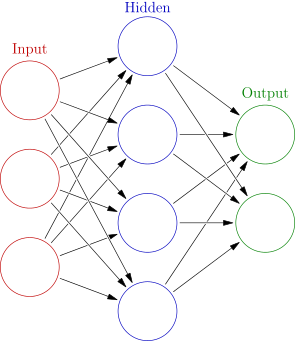
\includegraphics{/img/entries/dependent-haskell-1/ffneural.png}
\caption{Feed-forward ANN architecture}
\end{figure}

Here's a quick run through on background for ANN's --- but remember, this isn't
an article on ANN's, so we are going to be glossing over some of the details.

We're going to be implementing a \emph{feed-forward neural network} with
back-propagation training. These networks are layers of ``nodes'', each
connected to the each of the nodes of the previous layer. Input goes to the
first layer, which feeds information to the next layer, which feeds it to the
next, etc., until the final layer, where we read it off as the ``answer'' that
the network is giving us. Layers between the input and output layers are called
\emph{hidden} layers. Every node ``outputs'' a weighted sum of all of the
outputs of the \emph{previous} layer, plus an always-on ``bias'' term (so that
its result can be non-zero even when all of its inputs are zero). Symbolically,
it looks like:

\[
y_j = b_j + \sum_i^m w_{ij} x_i
\]

Or, if we treat the output of a layer and the list of list of weights as a
matrix, we can write it a little cleaner:

\[
\mathbf{y} = \mathbf{b} + W \mathbf{x}
\]

The result, the \(n\)-vector of nodes \(\mathbf{y}\), is computed from the
\(n\)-vector of biases \(\mathbf{b}\) and the \(n \times m\) weight matrix \(W\)
multiplied with the \(m\)-vector input, \(\mathbf{x}\).

To ``scale'' the result (and to give the system the magical powers of
nonlinearity), we actually apply an ``activation function'' to the output before
passing it down to the next step. We'll be using the popular
\href{https://en.wikipedia.org/wiki/Logistic_function}{logistic function},
\(f(x) = 1 / (1 + e^{-x})\).

\emph{Training} a network involves picking the right set of weights to get the
network to answer the question you want.

\section{Vanilla Types}\label{vanilla-types}

We can store a network by storing the matrix of of weights and biases between
each layer:

\begin{Shaded}
\begin{Highlighting}[]
\CommentTok{{-}{-} source: https://github.com/mstksg/inCode/tree/master/code{-}samples/dependent{-}haskell/NetworkUntyped.hs\#L18{-}L20}

\KeywordTok{data} \DataTypeTok{Weights} \OtherTok{=} \DataTypeTok{W}\NormalTok{ \{}\OtherTok{ wBiases ::} \OperatorTok{!}\NormalTok{(}\DataTypeTok{Vector} \DataTypeTok{Double}\NormalTok{)  }\CommentTok{{-}{-} n}
\NormalTok{                 ,}\OtherTok{ wNodes  ::} \OperatorTok{!}\NormalTok{(}\DataTypeTok{Matrix} \DataTypeTok{Double}\NormalTok{)  }\CommentTok{{-}{-} n x m}
\NormalTok{                 \}                              }\CommentTok{{-}{-} "m to n" layer}
\end{Highlighting}
\end{Shaded}

Now, a \texttt{Weights} linking an \emph{m}-node layer to an \emph{n}-node layer
has an \emph{n}-dimensional bias vector (one component for each output) and an
\emph{n}-by-\emph{m} node weight matrix (one column for each output, one row for
each input).

(We're using the \texttt{Matrix} type from the awesome
\emph{\href{http://hackage.haskell.org/package/hmatrix}{hmatrix}} library for
performant linear algebra, implemented using blas/lapack under the hood)

A feed-forward neural network is then just a linked list of these weights:

\begin{Shaded}
\begin{Highlighting}[]
\CommentTok{{-}{-} source: https://github.com/mstksg/inCode/tree/master/code{-}samples/dependent{-}haskell/NetworkUntyped.hs\#L22{-}L28}

\KeywordTok{data} \DataTypeTok{Network}\OtherTok{ ::} \OperatorTok{*} \KeywordTok{where}
    \DataTypeTok{O}\OtherTok{     ::} \OperatorTok{!}\DataTypeTok{Weights}
          \OtherTok{{-}\textgreater{}} \DataTypeTok{Network}
\OtherTok{    (:\&\textasciitilde{}) ::} \OperatorTok{!}\DataTypeTok{Weights}
          \OtherTok{{-}\textgreater{}} \OperatorTok{!}\DataTypeTok{Network}
          \OtherTok{{-}\textgreater{}} \DataTypeTok{Network}
\KeywordTok{infixr} \DecValTok{5} \OperatorTok{:\&\textasciitilde{}}
\end{Highlighting}
\end{Shaded}

Note that we're using \href{https://en.wikibooks.org/wiki/Haskell/GADT}{GADT}
syntax here, which just lets us define \texttt{Network} (with a kind signature,
\texttt{*}) by providing the type of its \emph{constructors}, \texttt{O} and
\texttt{(:\&\textasciitilde{})}. It'd be equivalent to the following normal data
declaration:

\begin{Shaded}
\begin{Highlighting}[]
\KeywordTok{data} \DataTypeTok{Network} \OtherTok{=} \DataTypeTok{O} \DataTypeTok{Weights}
             \OperatorTok{|} \DataTypeTok{Weights} \OperatorTok{:\&\textasciitilde{}} \DataTypeTok{Network}
\end{Highlighting}
\end{Shaded}

A network with one input layer, two inner layers, and one output layer would
look like:

\begin{Shaded}
\begin{Highlighting}[]
\NormalTok{ih }\OperatorTok{:\&\textasciitilde{}}\NormalTok{ hh }\OperatorTok{:\&\textasciitilde{}} \DataTypeTok{O}\NormalTok{ ho}
\end{Highlighting}
\end{Shaded}

The first component is the weights from the input to first inner layer, the
second is the weights between the two hidden layers, and the last is the weights
between the last hidden layer and the output layer.

We can write simple procedures, like generating random networks:

\begin{Shaded}
\begin{Highlighting}[]
\CommentTok{{-}{-} source: https://github.com/mstksg/inCode/tree/master/code{-}samples/dependent{-}haskell/NetworkUntyped.hs\#L46{-}L56}

\OtherTok{randomWeights ::} \DataTypeTok{MonadRandom}\NormalTok{ m }\OtherTok{=\textgreater{}} \DataTypeTok{Int} \OtherTok{{-}\textgreater{}} \DataTypeTok{Int} \OtherTok{{-}\textgreater{}}\NormalTok{ m }\DataTypeTok{Weights}
\NormalTok{randomWeights i o }\OtherTok{=} \KeywordTok{do}
\OtherTok{    seed1 ::} \DataTypeTok{Int} \OtherTok{\textless{}{-}}\NormalTok{ getRandom}
\OtherTok{    seed2 ::} \DataTypeTok{Int} \OtherTok{\textless{}{-}}\NormalTok{ getRandom}
    \KeywordTok{let}\NormalTok{ wB }\OtherTok{=}\NormalTok{ randomVector  seed1 }\DataTypeTok{Uniform}\NormalTok{ o }\OperatorTok{*} \DecValTok{2} \OperatorTok{{-}} \DecValTok{1}
\NormalTok{        wN }\OtherTok{=}\NormalTok{ uniformSample seed2 o (}\FunctionTok{replicate}\NormalTok{ i (}\OperatorTok{{-}}\DecValTok{1}\NormalTok{, }\DecValTok{1}\NormalTok{))}
    \FunctionTok{return} \OperatorTok{$} \DataTypeTok{W}\NormalTok{ wB wN}

\OtherTok{randomNet ::} \DataTypeTok{MonadRandom}\NormalTok{ m }\OtherTok{=\textgreater{}} \DataTypeTok{Int} \OtherTok{{-}\textgreater{}}\NormalTok{ [}\DataTypeTok{Int}\NormalTok{] }\OtherTok{{-}\textgreater{}} \DataTypeTok{Int} \OtherTok{{-}\textgreater{}}\NormalTok{ m }\DataTypeTok{Network}
\NormalTok{randomNet i []     o }\OtherTok{=}     \DataTypeTok{O} \OperatorTok{\textless{}$\textgreater{}}\NormalTok{ randomWeights i o}
\NormalTok{randomNet i (h}\OperatorTok{:}\NormalTok{hs) o }\OtherTok{=}\NormalTok{ (}\OperatorTok{:\&\textasciitilde{}}\NormalTok{) }\OperatorTok{\textless{}$\textgreater{}}\NormalTok{ randomWeights i h }\OperatorTok{\textless{}*\textgreater{}}\NormalTok{ randomNet h hs o}
\end{Highlighting}
\end{Shaded}

(We're using the \texttt{MonadRandom} typeclass from the
\emph{\href{http://hackage.haskell.org/package/MonadRandom}{MonadRandom}}
library, which uses the mechanisms in
\emph{\href{http://hackage.haskell.org/package/random-1.1/docs/System-Random.html}{System.Random}}
and gives us a generic way of working with monads where we can get random values
with \texttt{getRandom}, etc.)

(\href{http://hackage.haskell.org/package/hmatrix-0.17.0.1/docs/Numeric-LinearAlgebra.html\#v:randomVector}{\texttt{randomVector}}
and
\href{http://hackage.haskell.org/package/hmatrix-0.17.0.1/docs/Numeric-LinearAlgebra.html\#v:uniformSample}{\texttt{uniformSample}}
are from the \emph{\href{http://hackage.haskell.org/package/hmatrix}{hmatrix}}
library, generating random vectors and matrices from a random \texttt{Int} seed.
We manipulate them here to generate them with numbers between -1 and 1)

And now we can write a function to ``run'' our network on a given input vector,
following the matrix equation we wrote earlier:

\begin{Shaded}
\begin{Highlighting}[]
\CommentTok{{-}{-} source: https://github.com/mstksg/inCode/tree/master/code{-}samples/dependent{-}haskell/NetworkUntyped.hs\#L30{-}L44}

\OtherTok{logistic ::} \DataTypeTok{Floating}\NormalTok{ a }\OtherTok{=\textgreater{}}\NormalTok{ a }\OtherTok{{-}\textgreater{}}\NormalTok{ a}
\NormalTok{logistic x }\OtherTok{=} \DecValTok{1} \OperatorTok{/}\NormalTok{ (}\DecValTok{1} \OperatorTok{+} \FunctionTok{exp}\NormalTok{ (}\OperatorTok{{-}}\NormalTok{x))}

\OtherTok{runLayer ::} \DataTypeTok{Weights} \OtherTok{{-}\textgreater{}} \DataTypeTok{Vector} \DataTypeTok{Double} \OtherTok{{-}\textgreater{}} \DataTypeTok{Vector} \DataTypeTok{Double}
\NormalTok{runLayer (}\DataTypeTok{W}\NormalTok{ wB wN) v }\OtherTok{=}\NormalTok{ wB }\OperatorTok{+}\NormalTok{ wN }\OperatorTok{\#\textgreater{}}\NormalTok{ v}

\OtherTok{runNet ::} \DataTypeTok{Network} \OtherTok{{-}\textgreater{}} \DataTypeTok{Vector} \DataTypeTok{Double} \OtherTok{{-}\textgreater{}} \DataTypeTok{Vector} \DataTypeTok{Double}
\NormalTok{runNet (}\DataTypeTok{O}\NormalTok{ w)      }\OperatorTok{!}\NormalTok{v }\OtherTok{=}\NormalTok{ logistic (runLayer w v)}
\NormalTok{runNet (w }\OperatorTok{:\&\textasciitilde{}}\NormalTok{ n\textquotesingle{}) }\OperatorTok{!}\NormalTok{v }\OtherTok{=} \KeywordTok{let}\NormalTok{ v\textquotesingle{} }\OtherTok{=}\NormalTok{ logistic (runLayer w v)}
                       \KeywordTok{in}\NormalTok{  runNet n\textquotesingle{} v\textquotesingle{}}
\end{Highlighting}
\end{Shaded}

(\texttt{\#\textgreater{}} is matrix-vector multiplication)

If you're a non-Haskell programmer, this might all seem perfectly fine and
normal, and you probably have only a slightly elevated heart rate. If you are a
Haskell programmer, you are most likely already having heart attacks. Let's
imagine all of the bad things that could happen:

\begin{itemize}
\item
  How do we know that we didn't accidentally mix up the dimensions for our
  implementation of \texttt{randomWeights}? We could have switched parameters
  and be none the wiser.
\item
  How do we even know that each subsequent matrix in the network is
  ``compatible''? We want the outputs of one matrix to line up with the inputs
  of the next, but there's no way to know. It's possible to build a bad network,
  and things will just explode at runtime.
\item
  How do we know the size of vector the network expects? What stops you from
  sending in a bad vector at run-time? We might do runtime-checks, but the
  compiler won't help us.
\item
  How do we verify that we have implemented \texttt{runLayer} and
  \texttt{runNet} in a way that they won't suddenly fail at runtime? We write
  \texttt{l\ \#\textgreater{}\ v}, but how do we know that it's even
  correct\ldots what if we forgot to multiply something, or used something in
  the wrong places? We can it prove ourselves, but the compiler won't help us.
\end{itemize}

\subsection{Back-propagation}\label{back-propagation}

Now, let's try implementing back-propagation! It's a textbook gradient descent
algorithm. There are \href{https://en.wikipedia.org/wiki/Backpropagation}{many
explanations} on the internet; the basic idea is that you try to minimize the
squared error of what the neural network outputs for a given input vs.~the
actual expected output. You find the direction of change that minimizes the
error (by finding the derivative), and move that direction. The implementation
of backpropagation is found in many sources online and in literature, so let's
see the implementation in Haskell:

\begin{Shaded}
\begin{Highlighting}[]
\CommentTok{{-}{-} source: https://github.com/mstksg/inCode/tree/master/code{-}samples/dependent{-}haskell/NetworkUntyped.hs\#L58{-}L96}

\OtherTok{train ::} \DataTypeTok{Double}           \CommentTok{{-}{-} \^{} learning rate}
      \OtherTok{{-}\textgreater{}} \DataTypeTok{Vector} \DataTypeTok{Double}    \CommentTok{{-}{-} \^{} input vector}
      \OtherTok{{-}\textgreater{}} \DataTypeTok{Vector} \DataTypeTok{Double}    \CommentTok{{-}{-} \^{} target vector}
      \OtherTok{{-}\textgreater{}} \DataTypeTok{Network}          \CommentTok{{-}{-} \^{} network to train}
      \OtherTok{{-}\textgreater{}} \DataTypeTok{Network}
\NormalTok{train rate x0 target }\OtherTok{=} \FunctionTok{fst} \OperatorTok{.}\NormalTok{ go x0}
  \KeywordTok{where}
\OtherTok{    go ::} \DataTypeTok{Vector} \DataTypeTok{Double}    \CommentTok{{-}{-} \^{} input vector}
       \OtherTok{{-}\textgreater{}} \DataTypeTok{Network}          \CommentTok{{-}{-} \^{} network to train}
       \OtherTok{{-}\textgreater{}}\NormalTok{ (}\DataTypeTok{Network}\NormalTok{, }\DataTypeTok{Vector} \DataTypeTok{Double}\NormalTok{)}
    \CommentTok{{-}{-} handle the output layer}
\NormalTok{    go }\OperatorTok{!}\NormalTok{x (}\DataTypeTok{O}\NormalTok{ w}\OperatorTok{@}\NormalTok{(}\DataTypeTok{W}\NormalTok{ wB wN))}
        \OtherTok{=} \KeywordTok{let}\NormalTok{ y    }\OtherTok{=}\NormalTok{ runLayer w x}
\NormalTok{              o    }\OtherTok{=}\NormalTok{ logistic y}
              \CommentTok{{-}{-} the gradient (how much y affects the error)}
              \CommentTok{{-}{-}   (logistic\textquotesingle{} is the derivative of logistic)}
\NormalTok{              dEdy }\OtherTok{=}\NormalTok{ logistic\textquotesingle{} y }\OperatorTok{*}\NormalTok{ (o }\OperatorTok{{-}}\NormalTok{ target)}
              \CommentTok{{-}{-} new bias weights and node weights}
\NormalTok{              wB\textquotesingle{}  }\OtherTok{=}\NormalTok{ wB }\OperatorTok{{-}}\NormalTok{ scale rate dEdy}
\NormalTok{              wN\textquotesingle{}  }\OtherTok{=}\NormalTok{ wN }\OperatorTok{{-}}\NormalTok{ scale rate (dEdy }\OtherTok{\textasciigrave{}outer\textasciigrave{}}\NormalTok{ x)}
\NormalTok{              w\textquotesingle{}   }\OtherTok{=} \DataTypeTok{W}\NormalTok{ wB\textquotesingle{} wN\textquotesingle{}}
              \CommentTok{{-}{-} bundle of derivatives for next step}
\NormalTok{              dWs  }\OtherTok{=}\NormalTok{ tr wN }\OperatorTok{\#\textgreater{}}\NormalTok{ dEdy}
          \KeywordTok{in}\NormalTok{  (}\DataTypeTok{O}\NormalTok{ w\textquotesingle{}, dWs)}
    \CommentTok{{-}{-} handle the inner layers}
\NormalTok{    go }\OperatorTok{!}\NormalTok{x (w}\OperatorTok{@}\NormalTok{(}\DataTypeTok{W}\NormalTok{ wB wN) }\OperatorTok{:\&\textasciitilde{}}\NormalTok{ n)}
        \OtherTok{=} \KeywordTok{let}\NormalTok{ y          }\OtherTok{=}\NormalTok{ runLayer w x}
\NormalTok{              o          }\OtherTok{=}\NormalTok{ logistic y}
              \CommentTok{{-}{-} get dWs\textquotesingle{}, bundle of derivatives from rest of the net}
\NormalTok{              (n\textquotesingle{}, dWs\textquotesingle{}) }\OtherTok{=}\NormalTok{ go o n}
              \CommentTok{{-}{-} the gradient (how much y affects the error)}
\NormalTok{              dEdy       }\OtherTok{=}\NormalTok{ logistic\textquotesingle{} y }\OperatorTok{*}\NormalTok{ dWs\textquotesingle{}}
              \CommentTok{{-}{-} new bias weights and node weights}
\NormalTok{              wB\textquotesingle{}  }\OtherTok{=}\NormalTok{ wB }\OperatorTok{{-}}\NormalTok{ scale rate dEdy}
\NormalTok{              wN\textquotesingle{}  }\OtherTok{=}\NormalTok{ wN }\OperatorTok{{-}}\NormalTok{ scale rate (dEdy }\OtherTok{\textasciigrave{}outer\textasciigrave{}}\NormalTok{ x)}
\NormalTok{              w\textquotesingle{}   }\OtherTok{=} \DataTypeTok{W}\NormalTok{ wB\textquotesingle{} wN\textquotesingle{}}
              \CommentTok{{-}{-} bundle of derivatives for next step}
\NormalTok{              dWs  }\OtherTok{=}\NormalTok{ tr wN }\OperatorTok{\#\textgreater{}}\NormalTok{ dEdy}
          \KeywordTok{in}\NormalTok{  (w\textquotesingle{} }\OperatorTok{:\&\textasciitilde{}}\NormalTok{ n\textquotesingle{}, dWs)}
\end{Highlighting}
\end{Shaded}

The algorithm computes the \emph{updated} network by recursively updating the
layers, backwards up from the output layer. At every step, it returns the
updated layer/network, as well as a bundle of derivatives (\texttt{dWs}) for the
next layer up to use to calculate its descent direction.

At the output layer, all it needs to calculate the direction of descent is just
\texttt{o\ -\ targ}, the target. At the inner layers, it has to use the
\texttt{dWs} bundle it receives from the lower layers to figure it out.
\texttt{dWs} essentially ``bubbles up'' from the output layer up to the input
layer calculations.

Writing this is a bit of a struggle. I actually implemented this incorrectly
several times before writing it as you see here. The type system doesn't help
you like it normally does in Haskell, and you can't really use parametricity to
help you write your code like normal Haskell. Everything is monomorphic, and
everything multiplies with everything else. You don't have any hints about what
to multiply with what at any point in time. It's like all of the bad things
mentioned before, but amplified.

In short, you're leaving yourself open to many potential bugs\ldots and the
compiler doesn't help you write your code at all! This is the nightmare of every
Haskell programmer. There must be a better way!\footnote{This sentence is the
  story of my Haskell life.}

\subsubsection{Putting it to the test}\label{putting-it-to-the-test}

Pretty much the only way you can verify this code is to test it out on example
cases. In the
\href{https://github.com/mstksg/inCode/tree/master/code-samples/dependent-haskell/NetworkUntyped.hs}{source
file}, I have
\href{https://github.com/mstksg/inCode/tree/master/code-samples/dependent-haskell/NetworkUntyped.hs\#L128-L136}{\texttt{main}}
test out the backprop, training a network on a 2D function that was ``on'' for
two small circles and ``off'' everywhere else (A nice cute
non-linearly-separable function to test our network on). We basically train the
network to be able to recognize the two-circle pattern. I implemented a simple
printing function and tested the trained network on a grid:

\begin{Shaded}
\begin{Highlighting}[]
\ExtensionTok{$}\NormalTok{ stack install hmatrix MonadRandom}
\ExtensionTok{$}\NormalTok{ stack ghc }\AttributeTok{{-}{-}} \AttributeTok{{-}O2}\NormalTok{ ./NetworkUntyped.hs}
\ExtensionTok{$}\NormalTok{ ./NetworkUntyped}
\CommentTok{\# Training network...}
\CommentTok{\#}
\CommentTok{\#}
\CommentTok{\#            .=\#\#\#\#\#\#\#\#=}
\CommentTok{\#          .\#\#\#\#\#\#\#\#\#\#\#\#\#\#.}
\CommentTok{\#          \#\#\#\#\#\#\#\#\#\#\#\#\#\#\#\#}
\CommentTok{\#          \#\#\#\#\#\#\#\#\#\#\#\#\#\#\#\#}
\CommentTok{\#          .\#\#\#\#\#\#\#\#\#\#\#\#\#\#{-}}
\CommentTok{\#            .\#\#\#\#\#\#\#\#\#\#\#}
\CommentTok{\#                 ...             ...}
\CommentTok{\#                             {-}\#\#\#\#\#\#\#\#\#\#.}
\CommentTok{\#                           {-}\#\#\#\#\#\#\#\#\#\#\#\#\#\#.}
\CommentTok{\#                           \#\#\#\#\#\#\#\#\#\#\#\#\#\#\#\#}
\CommentTok{\#                           \#\#\#\#\#\#\#\#\#\#\#\#\#\#\#\#}
\CommentTok{\#                            =\#\#\#\#\#\#\#\#\#\#\#\#=}
\CommentTok{\#                              .\#\#\#\#\#\#\#=.}
\CommentTok{\#}
\CommentTok{\#}
\end{Highlighting}
\end{Shaded}

Not too bad! The network learned to recognize the circles. But, I was basically
forced to resort to unit testing to ensure my code was correct. Let's see if we
can do better.

\subsection{The Call of Types}\label{the-call-of-types}

Before we go on to the ``typed'' version of our program, let's take a step back
and look at some big checks you might want to ask yourself after you write code
in Haskell.

\begin{enumerate}
\def\labelenumi{\arabic{enumi}.}
\tightlist
\item
  Are any of my functions either partial or implemented using partial functions?
\item
  How could I have written things that are \emph{incorrect}, and yet still type
  check? Where does the compiler \emph{not} help me by restricting my choices?
\end{enumerate}

Both of these questions usually yield some truth about the code you write and
the things you should worry about. As a Haskeller, they should always be at the
back of your mind!

Looking back at our untyped implementation, we notice some things:

\begin{enumerate}
\def\labelenumi{\arabic{enumi}.}
\tightlist
\item
  Literally every single function we wrote is partial. Like,
  actually.\footnote{Okay, maybe not \emph{literally} every one. But, pretty
    much every one.} If we had passed in the incorrectly sized matrix/vector, or
  stored mismatched vectors in our network, everything would fall apart.
\item
  There are billions of ways we could have implemented our functions where they
  would still typechecked. We could multiply mismatched matrices, or forget to
  multiply a matrix, etc.
\end{enumerate}

\section{With Static Size-Indexed Types}\label{with-static-size-indexed-types}

\subsection{Networks}\label{networks}

Gauging our potential problems, it seems like the first major class of bugs we
can address is improperly sized and incompatible matrices. If the compiler
always made sure we used compatible matrices, we can avoid bugs at compile-time,
and we also can get a friendly helper when we write programs (by knowing what
works with what, and what we need were, and helping us organize our logic)

Let's write a \texttt{Weights} type that tells you the size of its output and
the input it expects. Let's have, say, a \texttt{Weights\ 10\ 5} be a set of
weights that takes you from a layer of 10 nodes to a layer of 5 nodes.
\texttt{w\ ::\ Weights\ 4\ 6} would take you from a layer of 4 nodes to a layer
of 6 nodes:

\begin{Shaded}
\begin{Highlighting}[]
\CommentTok{{-}{-} source: https://github.com/mstksg/inCode/tree/master/code{-}samples/dependent{-}haskell/NetworkTyped.hs\#L21{-}L23}

\KeywordTok{data} \DataTypeTok{Weights}\NormalTok{ i o }\OtherTok{=} \DataTypeTok{W}\NormalTok{ \{}\OtherTok{ wBiases ::} \OperatorTok{!}\NormalTok{(}\DataTypeTok{R}\NormalTok{ o)}
\NormalTok{                     ,}\OtherTok{ wNodes  ::} \OperatorTok{!}\NormalTok{(}\DataTypeTok{L}\NormalTok{ o i)}
\NormalTok{                     \}                      }\CommentTok{{-}{-} an "o x i" layer}
\end{Highlighting}
\end{Shaded}

The type constructor \texttt{Weights} has the kind
\texttt{Weights\ ::\ Nat\ -\textgreater{}\ Nat\ -\textgreater{}\ *} --- it takes
two types of kind \texttt{Nat} (from the
\emph{\href{http://hackage.haskell.org/package/base-4.8.2.0/docs/GHC-TypeLits.html}{GHC.TypeLits}}
module, which the integer type literals give us with
\emph{\href{https://www.schoolofhaskell.com/user/konn/prove-your-haskell-for-great-safety/dependent-types-in-haskell\#type-level-naturals}{DataKinds}}
enabled) and returns a \texttt{*} --- a ``normal type''.

We're using the
\emph{\href{http://mstksg.github.io/hmatrix/Numeric-LinearAlgebra-Static.html}{Numeric.LinearAlgebra.Static}}
module from \emph{\href{http://hackage.haskell.org/package/hmatrix}{hmatrix}},
which offers matrix and vector types with their size in their types: an
\texttt{R\ 5} is a vector of Doubles with 5 elements, and a \texttt{L\ 3\ 6} is
a 3x6 vector of Doubles.

These types are called ``dependent'' types because the type itself
\emph{depends} on its value. If an \texttt{R\ n} contains a 5-element vector,
its type is \texttt{R\ 5}.

The \emph{Static} module in \emph{hmatrix} relies on the
\href{http://hackage.haskell.org/package/base-4.8.2.0/docs/GHC-TypeLits.html\#t:KnownNat}{\texttt{KnownNat}}
mechanism that GHC offers. Almost all operations in the library require a
\texttt{KnownNat} constraint on the type-level Nats --- for example, you can
take the dot product of two vectors with
\texttt{dot\ ::\ KnownNat\ n\ =\textgreater{}\ R\ n\ -\textgreater{}\ R\ n\ -\textgreater{}\ Double}.
It lets the library use the information in the \texttt{n} at runtime as an
\texttt{Integer}. (More on this later!)

Moving on, our network type for this post will be something like
\texttt{Network\ 10\ \textquotesingle{}{[}7,5,3{]}\ 2}: Take 10 inputs, return 2
outputs --- and internally, have hidden layers of size 7, 5, and 3. (The
\texttt{\textquotesingle{}{[}7,5,3{]}} is a type-level list of Nats; the
optional \texttt{\textquotesingle{}} apostrophe is just for our own benefit to
distinguish it from a value-level list of integers.)

\begin{Shaded}
\begin{Highlighting}[]
\CommentTok{{-}{-} source: https://github.com/mstksg/inCode/tree/master/code{-}samples/dependent{-}haskell/NetworkTyped.hs\#L25{-}L32}

\KeywordTok{data} \DataTypeTok{Network}\OtherTok{ ::} \DataTypeTok{Nat} \OtherTok{{-}\textgreater{}}\NormalTok{ [}\DataTypeTok{Nat}\NormalTok{] }\OtherTok{{-}\textgreater{}} \DataTypeTok{Nat} \OtherTok{{-}\textgreater{}} \OperatorTok{*} \KeywordTok{where}
    \DataTypeTok{O}\OtherTok{     ::} \OperatorTok{!}\NormalTok{(}\DataTypeTok{Weights}\NormalTok{ i o)}
          \OtherTok{{-}\textgreater{}} \DataTypeTok{Network}\NormalTok{ i \textquotesingle{}[] o}
\OtherTok{    (:\&\textasciitilde{}) ::} \DataTypeTok{KnownNat}\NormalTok{ h}
          \OtherTok{=\textgreater{}} \OperatorTok{!}\NormalTok{(}\DataTypeTok{Weights}\NormalTok{ i h)}
          \OtherTok{{-}\textgreater{}} \OperatorTok{!}\NormalTok{(}\DataTypeTok{Network}\NormalTok{ h hs o)}
          \OtherTok{{-}\textgreater{}} \DataTypeTok{Network}\NormalTok{ i (h \textquotesingle{}}\OperatorTok{:}\NormalTok{ hs) o}
\KeywordTok{infixr} \DecValTok{5} \OperatorTok{:\&\textasciitilde{}}
\end{Highlighting}
\end{Shaded}

We use GADT syntax here again. The \emph{kind signature} of the type constructor
means that the \texttt{Network} type constructor takes three inputs: a
\texttt{Nat} (type-level numeral, like \texttt{10} or \texttt{5}), list of
\texttt{Nat}s, and another \texttt{Nat} (the input, hidden layers, and output
sizes). Let's go over the two constructors.

\begin{itemize}
\item
  The \texttt{O} constructor takes a \texttt{Weights\ i\ o} and returns a
  \texttt{Network\ i\ \textquotesingle{}{[}{]}\ o}. That is, if your network is
  just weights from \texttt{i} inputs to \texttt{o} outputs, your network itself
  just takes \texttt{i} inputs and returns \texttt{o} outputs, with no hidden
  layers.
\item
  The \texttt{(:\&\textasciitilde{})} constructor takes a
  \texttt{Network\ h\ hs\ o} -- a network with \texttt{h} inputs and \texttt{o}
  outputs -- and ``conses'' an extra input layer in front. If you give it a
  \texttt{Weights\ i\ h}, its outputs fit perfectly into the inputs of the
  subnetwork, and you get a
  \texttt{Network\ i\ (h\ \textquotesingle{}:\ hs)\ o}.
  (\texttt{(\textquotesingle{}:)}, or \texttt{(:)}, is the same as normal
  \texttt{(:)}, but is for type-level lists. The apostrophe is optional here
  too, but it's just nice to be able to visually distinguish the two)

  We add a \texttt{KnownNat} constraint on the \texttt{h}, so that whenever you
  pattern match on \texttt{w\ :\&\textasciitilde{}\ net}, you automatically get
  a \texttt{KnownNat} constraint for the input size of \texttt{net} (and the
  output of \texttt{w}) that the \emph{hmatrix} library can use.
\end{itemize}

We can still construct them the same way:

\begin{Shaded}
\begin{Highlighting}[]
\CommentTok{{-}{-} given:}
\OtherTok{ih ::} \DataTypeTok{Weights} \DecValTok{10} \DecValTok{7}
\OtherTok{hh ::} \DataTypeTok{Weights}  \DecValTok{7} \DecValTok{4}
\OtherTok{ho ::} \DataTypeTok{Weights}  \DecValTok{4} \DecValTok{2}

\CommentTok{{-}{-} we have:}
              \DataTypeTok{O}\OtherTok{ ho ::} \DataTypeTok{Network}  \DecValTok{4}\NormalTok{ \textquotesingle{}[] }\DecValTok{2}
\NormalTok{       hh }\OperatorTok{:\&\textasciitilde{}} \DataTypeTok{O}\OtherTok{ ho ::} \DataTypeTok{Network}  \DecValTok{7}\NormalTok{ \textquotesingle{}[}\DecValTok{4}\NormalTok{] }\DecValTok{2}
\NormalTok{ih }\OperatorTok{:\&\textasciitilde{}}\NormalTok{ hh }\OperatorTok{:\&\textasciitilde{}} \DataTypeTok{O}\OtherTok{ ho ::} \DataTypeTok{Network} \DecValTok{10}\NormalTok{ \textquotesingle{}[}\DecValTok{7}\NormalTok{,}\DecValTok{4}\NormalTok{] }\DecValTok{2}
\end{Highlighting}
\end{Shaded}

Note that the shape of the constructors requires all of the weight vectors to
``fit together''. \texttt{ih\ :\&\textasciitilde{}\ O\ ho} would be a type error
(feeding a 7-output layer to a 4-input layer). Also, if we ever pattern match on
\texttt{:\&\textasciitilde{}}, we know that the resulting matrices and vectors
are compatible!

One neat thing is that this approach is also self-documenting. I don't need to
specify what the dimensions are in the docs and trust the users to read it and
obey it. The types tell them! And if they don't listen, they get a compiler
error! (You should, of course, still provide reasonable documentation. But, in
this case, the compiler actually enforces your documentation's statements!)

Generating random weights and networks is even nicer now:

\begin{Shaded}
\begin{Highlighting}[]
\CommentTok{{-}{-} source: https://github.com/mstksg/inCode/tree/master/code{-}samples/dependent{-}haskell/NetworkTyped.hs\#L57{-}L64}

\OtherTok{randomWeights ::}\NormalTok{ (}\DataTypeTok{MonadRandom}\NormalTok{ m, }\DataTypeTok{KnownNat}\NormalTok{ i, }\DataTypeTok{KnownNat}\NormalTok{ o)}
              \OtherTok{=\textgreater{}}\NormalTok{ m (}\DataTypeTok{Weights}\NormalTok{ i o)}
\NormalTok{randomWeights }\OtherTok{=} \KeywordTok{do}
\OtherTok{    s1 ::} \DataTypeTok{Int} \OtherTok{\textless{}{-}}\NormalTok{ getRandom}
\OtherTok{    s2 ::} \DataTypeTok{Int} \OtherTok{\textless{}{-}}\NormalTok{ getRandom}
    \KeywordTok{let}\NormalTok{ wB }\OtherTok{=}\NormalTok{ randomVector  s1 }\DataTypeTok{Uniform} \OperatorTok{*} \DecValTok{2} \OperatorTok{{-}} \DecValTok{1}
\NormalTok{        wN }\OtherTok{=}\NormalTok{ uniformSample s2 (}\OperatorTok{{-}}\DecValTok{1}\NormalTok{) }\DecValTok{1}
    \FunctionTok{return} \OperatorTok{$} \DataTypeTok{W}\NormalTok{ wB wN}
\end{Highlighting}
\end{Shaded}

Notice that the \emph{Static} versions of
\href{http://mstksg.github.io/hmatrix/Numeric-LinearAlgebra-Static.html\#v:randomVector}{\texttt{randomVector}}
and
\href{http://mstksg.github.io/hmatrix/Numeric-LinearAlgebra-Static.html\#v:uniformSample}{\texttt{uniformSample}}
don't actually require the size of the vector/matrix you want as an input --
they just use \emph{type inference} to figure out what size you want! This is
the same process that
\href{http://hackage.haskell.org/package/base-4.8.2.0/docs/Prelude.html\#v:read}{\texttt{read}}
uses to figure out what type of thing you want to return. You would use
\texttt{randomVector\ s\ Uniform\ ::\ R\ 10}, and type inference would give you
a 10-element vector the same way \texttt{read\ "hello"\ ::\ Int} would give you
an \texttt{Int}.

It's important to note that it's much harder to implement this incorrectly.
Before, you could give the matrix the wrong dimensions (maybe you flipped the
parameters?), or gave the wrong parameter to the vector generator.

But here, you are guaranteed/forced to return the correctly sized vectors and
matrices. In fact, you \emph{don't even have to worry} about it --- it's handled
automatically by the magic of type inference\footnote{Thank you based
  Hindley-Milner.}! I consider this a very big victory. One of the whole points
of types is to give you less to ``worry about'', as a programmer. Here, we
completely eliminate an \emph{entire dimension} of programmer concern.

\subsubsection{Benefits to the user}\label{benefits-to-the-user}

Not only is this style nicer for you as the implementer, it's also very
beneficial for the \emph{user} of the function. Consider looking at the two
competing type signatures side-by-side:

\begin{Shaded}
\begin{Highlighting}[]
\OtherTok{randomWeights ::} \DataTypeTok{Int} \OtherTok{{-}\textgreater{}} \DataTypeTok{Int} \OtherTok{{-}\textgreater{}}\NormalTok{ m }\DataTypeTok{Weights}
\OtherTok{randomWeights ::}\NormalTok{               m (}\DataTypeTok{Weights}\NormalTok{ i o)}
\end{Highlighting}
\end{Shaded}

If you want to \emph{use} this function, you have to look up some things from
the documentation:

\begin{enumerate}
\def\labelenumi{\arabic{enumi}.}
\tightlist
\item
  What do the two arguments represent?
\item
  What \emph{order} is the function expecting these two arguments?
\item
  What will be the dimension of the result?
\end{enumerate}

These are three things you \emph{need} to look up in the documentation. There's
simply no way around it.

But, here, all of these questions are answered \emph{immediately}, just from the
type (which you can get from GHC, or from ghci). You don't need to worry about
arguments. You don't need to worry about what order the function is expecting
the arguments to be in. And you already know \emph{exactly} what the dimensions
of the result is, right in the type.

I often implement many of my functions in this style, even if the rest of my
program isn't intended to be dependently typed (I can just convert the type to a
``dumb'' type as soon as I get the result). All of these benefits come even when
the caller doesn't \emph{care} at all about dependently typed programming ---
it's just a better style of defining functions/offering an API!

\subsection{Singletons and Induction}\label{singletons-and-induction}

The code for the updated \texttt{randomNet} takes a bit of background to
understand, so let's take a quick detour through the concepts of singletons,
dependent pattern matching, and induction on dependent data types.\footnote{This
  entire section was previously written to use the
  \href{http://hackage.haskell.org/package/typelits-witnesses}{typelits-witnesses}
  library, but has now been re-written to use the canonical
  \href{https://hackage.haskell.org/package/singletons}{singletons} library
  after a
  \href{https://www.reddit.com/r/haskell/comments/4l199z/practical_dependent_types_in_haskell_type_safe/d3jkslv}{conversation}
  with Andras Kovacs. The
  \href{https://github.com/mstksg/inCode/blob/697c1f726b9ab9c3f9830ed5521bfeee6ec10727/entry/practical-dependent-types-in-haskell-1.md\#singletons-and-induction}{old
  version} is still online at github, if you want to look at it or compare!}

Let's say we want to implement an algorithm that can create any
\texttt{Network\ i\ hs\ o}, so that we can construct a
\texttt{Network\ 4\ \textquotesingle{}{[}3,2{]}\ 1} or something. In true
Haskell fashion, we want do this recursively (``inductively''). After all, we
know how to make a \texttt{Network\ i\ \textquotesingle{}{[}{]}\ o} (just
\texttt{O\ \textless{}\$\textgreater{}\ randomWeights}), and we know how to
create a \texttt{Network\ i\ (h\ \textquotesingle{}:\ hs)\ o} if we had a
\texttt{Network\ h\ hs\ o} (just use \texttt{(:\&\textasciitilde{})} with
\texttt{randomWeights}). Now all we have to do is just ``pattern match'' on the
type-level list, and\ldots{}

Oh wait. We can't pattern match on types like that in Haskell. This is a
consequence of one of Haskell's fundamental design decisions: types are
\textbf{erased} at runtime. We need to have a way to ``access'' the type (at
run-time) as a \emph{value} so we can pattern match on it and do things with it.

In Haskell, the popular way to deal with this is by using \emph{singletons} ---
(parameterized) types which only have valid constructor. The canonical method of
working with singletons in Haskell is with the
\emph{\href{https://hackage.haskell.org/package/singletons}{singletons}}
library, which provides a uniform interface for all sorts of singletons of types
you'll encounter in everyday use.

We want to ``pattern match'' on a type-level list, so we want a singleton for
lists. The \emph{singletons} library provides them:

\begin{Shaded}
\begin{Highlighting}[]
\DataTypeTok{SNil}\OtherTok{  ::} \DataTypeTok{Sing}\NormalTok{ \textquotesingle{}[]}
\DataTypeTok{SCons}\OtherTok{ ::} \DataTypeTok{Sing}\NormalTok{ a }\OtherTok{{-}\textgreater{}} \DataTypeTok{Sing}\NormalTok{ as }\OtherTok{{-}\textgreater{}} \DataTypeTok{Sing}\NormalTok{ (a \textquotesingle{}}\OperatorTok{:}\NormalTok{ as)}
\end{Highlighting}
\end{Shaded}

This means that if we ever get value of type \texttt{Sing\ as} (and \texttt{as}
is a type-level list), we can pattern match on it. If we match on the
\texttt{SNil} constructor, we \emph{know} it's a
\texttt{Sing\ \textquotesingle{}{[}{]}} in that branch, and if we match on the
\texttt{SCons} constructor, we \emph{know} it's a
\texttt{Sing\ (a\ \textquotesingle{}:\ as)} -- a non-empty list. This is called
\emph{dependent pattern matching}. Every ``branch'' of your case statement has a
different inferred type of the arguments, depending on the constructor you match
on.

\begin{Shaded}
\begin{Highlighting}[]
\KeywordTok{case}\NormalTok{ foo }\KeywordTok{of}
  \DataTypeTok{SNil}      \OtherTok{{-}\textgreater{}} \OperatorTok{...}   \CommentTok{{-}{-} here, GHC knows \textasciigrave{}foo :: Sing \textquotesingle{}[]\textasciigrave{}}
  \DataTypeTok{SCons}\NormalTok{ \_ \_ }\OtherTok{{-}\textgreater{}} \OperatorTok{...}   \CommentTok{{-}{-} here, GHC knows \textasciigrave{}foo :: Sing (a \textquotesingle{}: as)\textasciigrave{}}
\end{Highlighting}
\end{Shaded}

\emph{singletons} actually provides a whole bunch of singleton constructors for
different types and kinds, like for \texttt{Bool}:

\begin{Shaded}
\begin{Highlighting}[]
\DataTypeTok{STrue}\OtherTok{  ::} \DataTypeTok{Sing} \DataTypeTok{\textquotesingle{}True}
\DataTypeTok{SFalse}\OtherTok{ ::} \DataTypeTok{Sing} \DataTypeTok{\textquotesingle{}False}
\end{Highlighting}
\end{Shaded}

(That's the \emph{type} \texttt{\textquotesingle{}True}, of \emph{kind}
\texttt{Bool})

So, if we ever are given a \texttt{Sing\ b} with some type-level \texttt{Bool}
we don't know, we can pattern match on it. And in the branch that \texttt{STrue}
matches on, \texttt{b} is \texttt{\textquotesingle{}True}, and in the branch
that \texttt{SFalse} matches on, \texttt{b} is \texttt{False}.

Singletons give us a way to pattern match on types by having an actual
term-level value we can pattern match on. So, we \emph{could} implement:

\begin{Shaded}
\begin{Highlighting}[]
\OtherTok{randomNet ::}\NormalTok{ (}\DataTypeTok{MonadRandom}\NormalTok{ m, }\DataTypeTok{KnownNat}\NormalTok{ i, }\DataTypeTok{KnownNat}\NormalTok{ o)}
          \OtherTok{=\textgreater{}} \DataTypeTok{Sing}\NormalTok{ hs }\OtherTok{{-}\textgreater{}}\NormalTok{ m (}\DataTypeTok{Network}\NormalTok{ i hs o)}
\end{Highlighting}
\end{Shaded}

And \texttt{randomNet} gets to directly pattern match and deconstruct on
\texttt{Sing\ hs}.

However, for actual API's, it's often more convenient to \emph{not} require the
extra parameter, and have it be ``inferred'' in the way we've been doing it
before. That way the \emph{user} doesn't have the burden of supplying it. The
\emph{singletons} library offers a typeclass we can use to implicitly conjure up
values of a singleton type -- \texttt{SingI}. We can use
\texttt{sing\ ::\ SingI\ s\ =\textgreater{}\ Sing\ s} to generate the
``inferred'' singleton:

\begin{Shaded}
\begin{Highlighting}[]
\NormalTok{ghci}\OperatorTok{\textgreater{}}\OtherTok{ sing ::} \DataTypeTok{Sing}\NormalTok{ \textquotesingle{}[]}
\DataTypeTok{SNil}
\NormalTok{ghci}\OperatorTok{\textgreater{}}\OtherTok{ sing ::} \DataTypeTok{Sing} \DataTypeTok{\textquotesingle{}True}
\DataTypeTok{STrue}
\NormalTok{ghci}\OperatorTok{\textgreater{}}\OtherTok{ sing ::} \DataTypeTok{Sing} \CharTok{\textquotesingle{}[\textquotesingle{}}\DataTypeTok{True}\NormalTok{, }\DataTypeTok{\textquotesingle{}False}\NormalTok{, }\DataTypeTok{\textquotesingle{}True}\NormalTok{]}
\DataTypeTok{STrue} \OtherTok{\textasciigrave{}SCons\textasciigrave{}} \DataTypeTok{SFalse} \OtherTok{\textasciigrave{}SCons\textasciigrave{}} \DataTypeTok{STrue} \OtherTok{\textasciigrave{}SCons\textasciigrave{}} \DataTypeTok{SNil}
\end{Highlighting}
\end{Shaded}

So if you have a function \texttt{SingI\ hs\ =\textgreater{}\ ...}, it's really
no different than \texttt{Sing\ hs\ -\textgreater{}\ ...}. The function itself
gets to use a \texttt{Sing\ hs} either way \ldots{} but for the first, the
argument is implicit.

The final piece of the puzzle is the singleton for a type-level \texttt{Nat}.
It's a little different because when you pattern match on it, instead of
directly learning about the type, you ``receive'' a \texttt{KnownNat} instance
you can use.

\begin{Shaded}
\begin{Highlighting}[]
\DataTypeTok{SNat}\OtherTok{ ::} \DataTypeTok{KnownNat}\NormalTok{ n }\OtherTok{=\textgreater{}} \DataTypeTok{Sing}\NormalTok{ n}
\end{Highlighting}
\end{Shaded}

\begin{Shaded}
\begin{Highlighting}[]
\CommentTok{{-}{-} \textasciigrave{}foo :: Sing n\textasciigrave{}, but we don\textquotesingle{}t know what \textasciigrave{}n\textasciigrave{} it is}
\KeywordTok{case}\NormalTok{ foo }\KeywordTok{of}
  \DataTypeTok{SNat} \OtherTok{{-}\textgreater{}} \OperatorTok{...}   \CommentTok{{-}{-} in this branch, we have a \textasciigrave{}KnownNat n\textasciigrave{} instance}
\end{Highlighting}
\end{Shaded}

Essentially, the data constructor comes ``packaged'' with a \texttt{KnownNat\ n}
instance. The \emph{creation} of \texttt{SNat\ ::\ Sing\ n} requires the
presence of \texttt{KnownNat\ n}. So if you ever pattern match on a validly
created \texttt{SNat}, the fact that that \texttt{SNat} constructor even exists
(instead of, say, being \texttt{undefined}) is a \emph{witness} to that very
\texttt{KnownNat} instance, and the type system lets us use this. It's as if you
``pattern match'' out the instance itself, like any other value the constructor
might have.

Now we have enough pieces of the puzzle:

\begin{Shaded}
\begin{Highlighting}[]
\CommentTok{{-}{-} source: https://github.com/mstksg/inCode/tree/master/code{-}samples/dependent{-}haskell/NetworkTyped.hs\#L66{-}L75}

\OtherTok{randomNet ::} \KeywordTok{forall}\NormalTok{ m i hs o}\OperatorTok{.}\NormalTok{ (}\DataTypeTok{MonadRandom}\NormalTok{ m, }\DataTypeTok{KnownNat}\NormalTok{ i, }\DataTypeTok{SingI}\NormalTok{ hs, }\DataTypeTok{KnownNat}\NormalTok{ o)}
          \OtherTok{=\textgreater{}}\NormalTok{ m (}\DataTypeTok{Network}\NormalTok{ i hs o)}
\NormalTok{randomNet }\OtherTok{=}\NormalTok{ go sing}
  \KeywordTok{where}
\OtherTok{    go ::} \KeywordTok{forall}\NormalTok{ h hs\textquotesingle{}}\OperatorTok{.} \DataTypeTok{KnownNat}\NormalTok{ h}
       \OtherTok{=\textgreater{}} \DataTypeTok{Sing}\NormalTok{ hs\textquotesingle{}}
       \OtherTok{{-}\textgreater{}}\NormalTok{ m (}\DataTypeTok{Network}\NormalTok{ h hs\textquotesingle{} o)}
\NormalTok{    go }\OtherTok{=}\NormalTok{ \textbackslash{}}\KeywordTok{case}
        \DataTypeTok{SNil}            \OtherTok{{-}\textgreater{}}     \DataTypeTok{O} \OperatorTok{\textless{}$\textgreater{}}\NormalTok{ randomWeights}
        \DataTypeTok{SNat} \OtherTok{\textasciigrave{}SCons\textasciigrave{}}\NormalTok{ ss }\OtherTok{{-}\textgreater{}}\NormalTok{ (}\OperatorTok{:\&\textasciitilde{}}\NormalTok{) }\OperatorTok{\textless{}$\textgreater{}}\NormalTok{ randomWeights }\OperatorTok{\textless{}*\textgreater{}}\NormalTok{ go ss}
\end{Highlighting}
\end{Shaded}

The real heavy lifting is done by \texttt{go} (written with
\href{https://www.schoolofhaskell.com/school/to-infinity-and-beyond/pick-of-the-week/guide-to-ghc-extensions/basic-syntax-extensions\#lambdacase}{LambdaCase}),
which takes the singleton structure it needs and recursively calls it until it
reaches the base case (\texttt{SNil}, an output layer). We just call
\texttt{go\ sing} to give it the initial structure it needs. Note there,
\texttt{sing\ ::\ Sing\ hs}, but this is inferred, because \texttt{go} is
\texttt{Sing\ hs\ -\textgreater{}\ Network\ i\ hs\ o}, and it's being asked to
return a \texttt{Network\ i\ hs\ o}, so it's safely inferable that we want
\texttt{Sing\ hs}.

Remember that we can write
\texttt{O\ \textless{}\$\textgreater{}\ randomWeights} because
\texttt{randomWeights}, like \texttt{read}, adapts to whatever type we want from
it --- in this case, we ask for a \texttt{Weights\ h\ o}, and type inference is
the real hero.

When possible, we like to write functions like \texttt{go} that take
\emph{explicit} singletons. In a lot of situations, we'll actually write our
internal \emph{logic} itself using explicit singletons, and only use
\texttt{SingI} and implicit singletons at the \emph{external} boundaries of our
API (like \texttt{randomNet}) for convenience to the user.

We've stumbled upon common pattern in dependent Haskell: ``building up'' a
value-level singleton \emph{structure} from a type that we want (either
explicitly given as an argument, or provided through a typeclass like
\texttt{SingI}) and then inductively piggybacking on that structure's
constructors to build the thing you \emph{really} want (called ``elimination'').
Here, we use \texttt{SingI\ hs} and ``eliminate'' that structure to create our
\texttt{Network\ i\ hs\ o}.

\subsubsection{On Typeclasses and
Dictionaries}\label{on-typeclasses-and-dictionaries}

One of the more bizarre things here, to me, is that \texttt{SNat} somehow gave
us a \texttt{KnownNat\ n} instance that we can use and pass off to
\texttt{randomWeights}. However, once you realize that typeclasses in Haskell
really aren't any more than a way to pass in implicit arguments, it starts to
make sense.

The only thing you can really do from a \texttt{KnownNat} is to get an
\texttt{Integer} from it with \texttt{natVal}. So really,
\texttt{KnownNat\ n\ =\textgreater{}\ ...} is more or less the same as
\texttt{Integer\ -\textgreater{}\ ...}. That's right --- at runtime, a
\texttt{KnownNat\ n} constraint is more or less just an \texttt{Integer} that
GHC passes around automatically for you, to save you the hassle of manually
passing it in yourself. (We say that the ``dictionary'' of \texttt{KnownNat} is
\texttt{Integer}.)

So, the constructor:

\begin{Shaded}
\begin{Highlighting}[]
\DataTypeTok{SNat}\OtherTok{ ::} \DataTypeTok{KnownNat}\NormalTok{ n }\OtherTok{=\textgreater{}} \DataTypeTok{Sing}\NormalTok{ n}
\end{Highlighting}
\end{Shaded}

Is really \emph{kind} of like:

\begin{Shaded}
\begin{Highlighting}[]
\DataTypeTok{SNat}\OtherTok{ ::} \DataTypeTok{Integer} \OtherTok{{-}\textgreater{}} \DataTypeTok{Sing}\NormalTok{ n}
\CommentTok{{-}{-} or, in normal data type notation}
\DataTypeTok{SNat} \DataTypeTok{Integer}
\CommentTok{{-}{-} kinda!}
\end{Highlighting}
\end{Shaded}

The GADT constructor for \texttt{SNat} requires a \texttt{KnownNat\ n} instance
in scope to produce. That instance is essentially stored inside the constructor
(as if it were just an \texttt{Integer}). Then, later, when you pattern match on
it, you pattern match out the instance that was originally put in there, and you
can use it!

So what's the big deal, why not just ditch \texttt{KnownNat} and just pass
around integers? The difference is that GHC and the compiler can now
\emph{track} these at compile-time to give you \emph{checks} on how your Nat's
act together on the type level, allowing it to catch mismatches with
compile-time checks instead of run-time checks.

\subsection{Running with it}\label{running-with-it}

So now, you can use
\texttt{randomNet\ ::\ IO\ (Network\ 5\ \textquotesingle{}{[}4,3{]}\ 2)} to get
a random network of the desired dimensions! (\texttt{IO} is an instance of
\texttt{MonadRandom})

Can we just pause right here to just appreciate how awesome it is that we can
generate random networks of whatever size we want by \emph{just requesting
something by its type}? Our implementation is also \emph{guaranteed} to have the
right sized matrices --- no worrying about using the right size parameters for
the right matrix in the right order. GHC does it for you automatically! And, for
the person who \emph{uses} \texttt{randomNet}, they don't have to bungle around
with figuring out what function argument indicates what, and in what order, and
they don't have to play a guessing game about the shape of the returned matrix.

The code for \emph{running} the nets is actually literally identical from
before:

\begin{Shaded}
\begin{Highlighting}[]
\CommentTok{{-}{-} source: https://github.com/mstksg/inCode/tree/master/code{-}samples/dependent{-}haskell/NetworkTyped.hs\#L42{-}L55}

\OtherTok{runLayer ::}\NormalTok{ (}\DataTypeTok{KnownNat}\NormalTok{ i, }\DataTypeTok{KnownNat}\NormalTok{ o)}
         \OtherTok{=\textgreater{}} \DataTypeTok{Weights}\NormalTok{ i o}
         \OtherTok{{-}\textgreater{}} \DataTypeTok{R}\NormalTok{ i}
         \OtherTok{{-}\textgreater{}} \DataTypeTok{R}\NormalTok{ o}
\NormalTok{runLayer (}\DataTypeTok{W}\NormalTok{ wB wN) v }\OtherTok{=}\NormalTok{ wB }\OperatorTok{+}\NormalTok{ wN }\OperatorTok{\#\textgreater{}}\NormalTok{ v}

\OtherTok{runNet ::}\NormalTok{ (}\DataTypeTok{KnownNat}\NormalTok{ i, }\DataTypeTok{KnownNat}\NormalTok{ o)}
       \OtherTok{=\textgreater{}} \DataTypeTok{Network}\NormalTok{ i hs o}
       \OtherTok{{-}\textgreater{}} \DataTypeTok{R}\NormalTok{ i}
       \OtherTok{{-}\textgreater{}} \DataTypeTok{R}\NormalTok{ o}
\NormalTok{runNet }\OtherTok{=}\NormalTok{ \textbackslash{}}\KeywordTok{case}
   \DataTypeTok{O}\NormalTok{ w }\OtherTok{{-}\textgreater{}}\NormalTok{ \textbackslash{}(}\OperatorTok{!}\NormalTok{v) }\OtherTok{{-}\textgreater{}}\NormalTok{ logistic (runLayer w v)}
\NormalTok{   (w }\OperatorTok{:\&\textasciitilde{}}\NormalTok{ n\textquotesingle{}) }\OtherTok{{-}\textgreater{}}\NormalTok{ \textbackslash{}(}\OperatorTok{!}\NormalTok{v) }\OtherTok{{-}\textgreater{}} \KeywordTok{let}\NormalTok{ v\textquotesingle{} }\OtherTok{=}\NormalTok{ logistic (runLayer w v)}
                          \KeywordTok{in}\NormalTok{ runNet n\textquotesingle{} v\textquotesingle{}}
\end{Highlighting}
\end{Shaded}

But now, we get the assurance that the matrices and vectors all fit each-other,
at compile-time. GHC basically writes our code for us. The operations all demand
vectors and matrices that ``fit together'', so you can only ever multiply a
matrix by a properly sized vector.

\begin{Shaded}
\begin{Highlighting}[]
\OtherTok{(+)  ::} \DataTypeTok{KnownNat}\NormalTok{ n}
     \OtherTok{=\textgreater{}} \DataTypeTok{R}\NormalTok{ n }\OtherTok{{-}\textgreater{}} \DataTypeTok{R}\NormalTok{ n }\OtherTok{{-}\textgreater{}} \DataTypeTok{R}\NormalTok{ n}
\OtherTok{(\#\textgreater{}) ::}\NormalTok{ (}\DataTypeTok{KnownNat}\NormalTok{ n, }\DataTypeTok{KnownNat}\NormalTok{ m)}
     \OtherTok{=\textgreater{}} \DataTypeTok{L}\NormalTok{ n m }\OtherTok{{-}\textgreater{}} \DataTypeTok{R}\NormalTok{ m }\OtherTok{{-}\textgreater{}} \DataTypeTok{R}\NormalTok{ n}

\OtherTok{logistic ::} \DataTypeTok{KnownNat}\NormalTok{ n}
         \OtherTok{=\textgreater{}} \DataTypeTok{R}\NormalTok{ n }\OtherTok{{-}\textgreater{}} \DataTypeTok{R}\NormalTok{ n}
\end{Highlighting}
\end{Shaded}

The source code is the same from before, so there isn't any extra overhead in
annotation. The correctness proofs and guarantees basically come without any
extra work --- they're free!

Our back-prop algorithm is ported pretty nicely too:

\begin{Shaded}
\begin{Highlighting}[]
\CommentTok{{-}{-} source: https://github.com/mstksg/inCode/tree/master/code{-}samples/dependent{-}haskell/NetworkTyped.hs\#L77{-}L116}

\OtherTok{train ::} \KeywordTok{forall}\NormalTok{ i hs o}\OperatorTok{.}\NormalTok{ (}\DataTypeTok{KnownNat}\NormalTok{ i, }\DataTypeTok{KnownNat}\NormalTok{ o)}
      \OtherTok{=\textgreater{}} \DataTypeTok{Double}           \CommentTok{{-}{-} \^{} learning rate}
      \OtherTok{{-}\textgreater{}} \DataTypeTok{R}\NormalTok{ i              }\CommentTok{{-}{-} \^{} input vector}
      \OtherTok{{-}\textgreater{}} \DataTypeTok{R}\NormalTok{ o              }\CommentTok{{-}{-} \^{} target vector}
      \OtherTok{{-}\textgreater{}} \DataTypeTok{Network}\NormalTok{ i hs o   }\CommentTok{{-}{-} \^{} network to train}
      \OtherTok{{-}\textgreater{}} \DataTypeTok{Network}\NormalTok{ i hs o}
\NormalTok{train rate x0 target }\OtherTok{=} \FunctionTok{fst} \OperatorTok{.}\NormalTok{ go x0}
  \KeywordTok{where}
\OtherTok{    go  ::} \KeywordTok{forall}\NormalTok{ j js}\OperatorTok{.} \DataTypeTok{KnownNat}\NormalTok{ j}
        \OtherTok{=\textgreater{}} \DataTypeTok{R}\NormalTok{ j              }\CommentTok{{-}{-} \^{} input vector}
        \OtherTok{{-}\textgreater{}} \DataTypeTok{Network}\NormalTok{ j js o   }\CommentTok{{-}{-} \^{} network to train}
        \OtherTok{{-}\textgreater{}}\NormalTok{ (}\DataTypeTok{Network}\NormalTok{ j js o, }\DataTypeTok{R}\NormalTok{ j)}
\NormalTok{    go }\OperatorTok{!}\NormalTok{x (}\DataTypeTok{O}\NormalTok{ w}\OperatorTok{@}\NormalTok{(}\DataTypeTok{W}\NormalTok{ wB wN))}
        \OtherTok{=} \KeywordTok{let}\NormalTok{ y    }\OtherTok{=}\NormalTok{ runLayer w x}
\NormalTok{              o    }\OtherTok{=}\NormalTok{ logistic y}
              \CommentTok{{-}{-} the gradient (how much y affects the error)}
              \CommentTok{{-}{-}   (logistic\textquotesingle{} is the derivative of logistic)}
\NormalTok{              dEdy }\OtherTok{=}\NormalTok{ logistic\textquotesingle{} y }\OperatorTok{*}\NormalTok{ (o }\OperatorTok{{-}}\NormalTok{ target)}
              \CommentTok{{-}{-} new bias weights and node weights}
\NormalTok{              wB\textquotesingle{}  }\OtherTok{=}\NormalTok{ wB }\OperatorTok{{-}}\NormalTok{ konst rate }\OperatorTok{*}\NormalTok{ dEdy}
\NormalTok{              wN\textquotesingle{}  }\OtherTok{=}\NormalTok{ wN }\OperatorTok{{-}}\NormalTok{ konst rate }\OperatorTok{*}\NormalTok{ (dEdy }\OtherTok{\textasciigrave{}outer\textasciigrave{}}\NormalTok{ x)}
\NormalTok{              w\textquotesingle{}   }\OtherTok{=} \DataTypeTok{W}\NormalTok{ wB\textquotesingle{} wN\textquotesingle{}}
              \CommentTok{{-}{-} bundle of derivatives for next step}
\NormalTok{              dWs  }\OtherTok{=}\NormalTok{ tr wN }\OperatorTok{\#\textgreater{}}\NormalTok{ dEdy}
          \KeywordTok{in}\NormalTok{  (}\DataTypeTok{O}\NormalTok{ w\textquotesingle{}, dWs)}
    \CommentTok{{-}{-} handle the inner layers}
\NormalTok{    go }\OperatorTok{!}\NormalTok{x (w}\OperatorTok{@}\NormalTok{(}\DataTypeTok{W}\NormalTok{ wB wN) }\OperatorTok{:\&\textasciitilde{}}\NormalTok{ n)}
        \OtherTok{=} \KeywordTok{let}\NormalTok{ y          }\OtherTok{=}\NormalTok{ runLayer w x}
\NormalTok{              o          }\OtherTok{=}\NormalTok{ logistic y}
              \CommentTok{{-}{-} get dWs\textquotesingle{}, bundle of derivatives from rest of the net}
\NormalTok{              (n\textquotesingle{}, dWs\textquotesingle{}) }\OtherTok{=}\NormalTok{ go o n}
              \CommentTok{{-}{-} the gradient (how much y affects the error)}
\NormalTok{              dEdy       }\OtherTok{=}\NormalTok{ logistic\textquotesingle{} y }\OperatorTok{*}\NormalTok{ dWs\textquotesingle{}}
              \CommentTok{{-}{-} new bias weights and node weights}
\NormalTok{              wB\textquotesingle{}  }\OtherTok{=}\NormalTok{ wB }\OperatorTok{{-}}\NormalTok{ konst rate }\OperatorTok{*}\NormalTok{ dEdy}
\NormalTok{              wN\textquotesingle{}  }\OtherTok{=}\NormalTok{ wN }\OperatorTok{{-}}\NormalTok{ konst rate }\OperatorTok{*}\NormalTok{ (dEdy }\OtherTok{\textasciigrave{}outer\textasciigrave{}}\NormalTok{ x)}
\NormalTok{              w\textquotesingle{}   }\OtherTok{=} \DataTypeTok{W}\NormalTok{ wB\textquotesingle{} wN\textquotesingle{}}
              \CommentTok{{-}{-} bundle of derivatives for next step}
\NormalTok{              dWs  }\OtherTok{=}\NormalTok{ tr wN }\OperatorTok{\#\textgreater{}}\NormalTok{ dEdy}
          \KeywordTok{in}\NormalTok{  (w\textquotesingle{} }\OperatorTok{:\&\textasciitilde{}}\NormalTok{ n\textquotesingle{}, dWs)}
\end{Highlighting}
\end{Shaded}

It's pretty much again almost an exact copy-and-paste, but now with GHC checking
to make sure everything fits together in our implementation.

One thing that's hard for me to convey here without walking through the
implementation step-by-step is how much the types \emph{help you} in writing
this code.

Before starting writing a back-prop implementation without the help of types,
I'd probably be a bit concerned. I mentioned earlier that writing the untyped
version was no fun at all. But, with the types, writing the implementation
became a \emph{joy} again. And, you have the help of \emph{hole driven
development}, too.

If you need, say, an \texttt{R\ n}, there might be only one way get it! And if
you have something that you need to combine with something you don't know about,
you can use typed holes (\texttt{\_}) and GHC will give you a list of all the
values you have in scope that can fit there. Your programs basically write
themselves!

The more you can restrict the implementations of your functions with your types,
the more of a joy programming in Haskell is. Things fit together and fall
together before your eyes\ldots and the best part is that if they're wrong, the
compiler will nudge you gently into the correct direction.

The most stressful part of programming happens when you have to tenuously hold a
complex and fragile network of ideas and constraints in your brain, and any
slight distraction or break in focus causes everything to crash down in your
mind. Over time, people have begun to believe that this is ``normal'' in
programming. Don't believe this lie --- it's \emph{not}! A good programming
experience involves maintaining as \emph{little} in your head as possible, and
letting the compiler handle remembering/checking the rest.

\subsubsection{The final test}\label{the-final-test}

You can download the
\href{https://github.com/mstksg/inCode/tree/master/code-samples/dependent-haskell/NetworkTyped.hs}{typed
network} source code and run it yourself. Again, the
\href{https://github.com/mstksg/inCode/tree/master/code-samples/dependent-haskell/NetworkTyped.hs\#L151-L159}{\texttt{main}}
method is written identically to that of the other file and tests the identical
function.

\begin{Shaded}
\begin{Highlighting}[]
\ExtensionTok{$}\NormalTok{ stack install hmatrix MonadRandom singletons}
\ExtensionTok{$}\NormalTok{ stack ghc }\AttributeTok{{-}{-}} \AttributeTok{{-}O2}\NormalTok{ ./NetworkTyped.hs}
\ExtensionTok{$}\NormalTok{ ./NetworkTyped}
\CommentTok{\# Training network...}
\CommentTok{\#}
\CommentTok{\#}
\CommentTok{\#             {-}\#\#\#\#\#\#\#\#\#{-}}
\CommentTok{\#           {-}\#\#\#\#\#\#\#\#\#\#\#\#\#=}
\CommentTok{\#          {-}\#\#\#\#\#\#\#\#\#\#\#\#\#\#\#{-}}
\CommentTok{\#          =\#\#\#\#\#\#\#\#\#\#\#\#\#\#\#=}
\CommentTok{\#           \#\#\#\#\#\#\#\#\#\#\#\#\#\#=.}
\CommentTok{\#            .\#\#\#\#\#\#\#\#\#\#=.}
\CommentTok{\#                               .==\#={-}}
\CommentTok{\#                            {-}\#\#\#\#\#\#\#\#\#\#\#{-}}
\CommentTok{\#                           =\#\#\#\#\#\#\#\#\#\#\#\#\#\#.}
\CommentTok{\#                          .\#\#\#\#\#\#\#\#\#\#\#\#\#\#\#=}
\CommentTok{\#                           =\#\#\#\#\#\#\#\#\#\#\#\#\#\#{-}}
\CommentTok{\#                            =\#\#\#\#\#\#\#\#\#\#\#\#{-}}
\CommentTok{\#                              {-}\#\#\#\#\#\#={-}.}
\CommentTok{\#}
\CommentTok{\#}
\end{Highlighting}
\end{Shaded}

\section{Finding Something to Depend on}\label{finding-something-to-depend-on}

We wrote out an initial ``non-typed'' implementation and recognized a lot red
flags that you might already be trained to recognize if you have been
programming Haskell for a while: \emph{partial functions} and \emph{multiple
potential implementations}.

We followed our well-tuned Haskell guts, listened to our hearts, and introduced
extra power in our types to remove all partial functions and eliminate
\emph{most} potential implementations (though not all, yet --- there are more
gains to be made from pulling in more parametric polymorphism).

Though we might have been able to find the bugs we avoided ``eventually'', we
were able to remove entire \emph{dimensions} of programmer concern and also
leverage parametric polymorphism to help write our programs for us. We found joy
again in programming.

In the process, however, we encountered some unexpected resistance from Haskell
(the language). We couldn't directly pattern match on our types, so we ended up
playing games with singletons and GADT constructors to pass instances.

In practice, using types as powerful and descriptive as these begin to require a
whole new set of tools once you get past the simplest use cases here. For
example, our \texttt{Network} types so far required you to specify their size in
the program itself (\texttt{Network\ 2\ \textquotesingle{}{[}16,\ 8{]}\ 1} in
the example source code, for instance). But what if we wanted to generate a
network that has runtime-determined size (For example, getting the size from
user input)? What if we wanted to load a pre-trained network whose size we don't
know? How can we manipulate our networks in a ``dynamic'' and generic way that
still gives us all of the benefits of type-safe programming? We'll found out
next post!

What we're looking at here is a world where \emph{types} can depend on run-time
values \ldots{} and values can depend on types. A world where types can be
returned from functions and where types become as much of a manipulatable
citizen of as values are.

The art of working with types like this is \emph{dependently typed programming}.
We're going to feel a bit of push back from Haskell at first, but after we hit
our stride and tame the tools we need, we're going to open up a whole new world
of potential!

\subsection{Exercises}\label{exercises}

Here are some exercises you can do for fun to test your understanding and apply
some of the concepts! The links are to the solutions in the source file.

\begin{enumerate}
\def\labelenumi{\arabic{enumi}.}
\item
  Write a function that
  \href{https://github.com/mstksg/inCode/tree/master/code-samples/dependent-haskell/NetworkTyped.hs\#L167-L168}{``pops''
  the input layer} off of a \texttt{Network}, returning both the input layer's
  weights and the rest of the network,
  \texttt{(Weights\ i\ h,\ Network\ h\ hs\ o)}.

  Think about what its type would have to be. Could it possibly be called with a
  network that cannot be popped? (that is, that has only one layer?)
\item
  Write a
  \href{https://github.com/mstksg/inCode/tree/master/code-samples/dependent-haskell/NetworkTyped.hs\#L170-L187}{function
  that takes two networks of the same dimensions and adds together their
  weights}. Remember that \texttt{L\ m\ n} has a \texttt{Num} instance that adds
  the matrices together element-by-element.

  Could this function ever be accidentally called on two networks that have
  different internal structures?
\item
  Write a function that takes a \texttt{Network\ i\ hs\ o} and
  \href{https://github.com/mstksg/inCode/tree/master/code-samples/dependent-haskell/NetworkTyped.hs\#L189-L192}{returns
  the singleton representing its hidden layer structure} --- \texttt{Sing\ hs}:

\begin{Shaded}
\begin{Highlighting}[]
\OtherTok{hiddenSing ::} \DataTypeTok{Network}\NormalTok{ i hs o }\OtherTok{{-}\textgreater{}} \DataTypeTok{Sing}\NormalTok{ hs}
\end{Highlighting}
\end{Shaded}

\begin{Shaded}
\begin{Highlighting}[]
\NormalTok{ghci}\OperatorTok{\textgreater{}}\NormalTok{ n }\OtherTok{\textless{}{-} randomNet ::} \DataTypeTok{IO}\NormalTok{ (}\DataTypeTok{Network} \DecValTok{10}\NormalTok{ \textquotesingle{}[}\DecValTok{5}\NormalTok{,}\DecValTok{3}\NormalTok{] }\DecValTok{1}\NormalTok{)}
\NormalTok{ghci}\OperatorTok{\textgreater{}} \KeywordTok{let}\NormalTok{ s }\OtherTok{=}\NormalTok{ hiddenSing n}
\NormalTok{ghci}\OperatorTok{\textgreater{}} \OperatorTok{:}\NormalTok{t s}
\OtherTok{s ::} \DataTypeTok{Sing}\NormalTok{ \textquotesingle{}[}\DecValTok{5}\NormalTok{,}\DecValTok{3}\NormalTok{]}
\NormalTok{ghci}\OperatorTok{\textgreater{}}\NormalTok{ s}
\DataTypeTok{SNat} \OtherTok{\textasciigrave{}SCons\textasciigrave{}} \DataTypeTok{SNat} \OtherTok{\textasciigrave{}SCons\textasciigrave{}} \DataTypeTok{SNil}
\end{Highlighting}
\end{Shaded}
\end{enumerate}

\section{Signoff}\label{signoff}

Hi, thanks for reading! You can reach me via email at
\href{mailto:justin@jle.im}{\nolinkurl{justin@jle.im}}, or at twitter at
\href{https://twitter.com/mstk}{@mstk}! This post and all others are published
under the \href{https://creativecommons.org/licenses/by-nc-nd/3.0/}{CC-BY-NC-ND
3.0} license. Corrections and edits via pull request are welcome and encouraged
at \href{https://github.com/mstksg/inCode}{the source repository}.

If you feel inclined, or this post was particularly helpful for you, why not
consider \href{https://www.patreon.com/justinle/overview}{supporting me on
Patreon}, or a \href{bitcoin:3D7rmAYgbDnp4gp4rf22THsGt74fNucPDU}{BTC donation}?
:)

\end{document}
